\documentclass{article}
\usepackage{geometry}
\geometry{margin=1in}
\usepackage{tikz}
\usepackage{amssymb}

\newif\ifsolutions
\solutionstrue % Show solutions
%\solutionsfalse % Hide solutions

% fleqn allows setting indent of display math
\usepackage[fleqn]{amsmath}
\setlength{\mathindent}{0pt} % Set indent
% Disable equation numbering (https://tex.stackexchange.com/a/360378)
\makeatletter
\renewcommand\tagform@[1]{}
\makeatother

% Allow Unicode (some, e.g., © and £ at least)
% https://tex.stackexchange.com/questions/370278/is-there-any-reason-to-use-inputenc
\usepackage[utf8]{inputenc}

% Hyperlinks
\usepackage{hyperref}
\hypersetup{colorlinks=true, urlcolor=blue, linkcolor=blue}

% Prevent indentation of paragraphs
\setlength\parindent{0pt}
\setlength{\parskip}{\baselineskip}

% Spacing above/below equations
% https://tex.stackexchange.com/a/69678
\AtBeginDocument{%
 \abovedisplayskip=-\parskip
 \abovedisplayshortskip=-\parskip
 \belowdisplayskip=0pt
 \belowdisplayshortskip=0pt
}

% Allow 3 additional subsection levels
% https://tex.stackexchange.com/a/60212
\usepackage{titlesec}
\setcounter{secnumdepth}{6}
% H4 in HTML
\titleformat{\paragraph}{\normalfont\normalsize\bfseries}{\theparagraph}{1em}{}
\titlespacing*{\paragraph}{0pt}{3.25ex plus 1ex minus .2ex}{1.5ex plus .2ex}
% H5 in HTML
\titleformat{\subparagraph}{\normalfont\normalsize\bfseries}{\thesubparagraph}{1em}{}
\titlespacing*{\subparagraph}{0pt}{3.25ex plus 1ex minus .2ex}{1.5ex plus .2ex}
% H6 in HTML
\titleformat{\subsubparagraph}{\normalfont\normalsize\bfseries}{\thesubsubparagraph}{1em}{}
\titlespacing*{\subsubparagraph}{0pt}{3.25ex plus 1ex minus .2ex}{1.5ex plus .2ex}

% So enumerate at all levels is numbers
% https://tex.stackexchange.com/questions/78842/nested-enumeration-numbering
\renewcommand{\labelenumii}{\arabic{enumii}.}
\renewcommand{\labelenumiii}{\arabic{enumiii}.}
\renewcommand{\labelenumiv}{\arabic{enumiv}.}

\renewcommand{\mbox}{\text}
\newcommand{\ds}[0]{\displaystyle}
\newcommand{\ihat}[0]{\hat{\boldsymbol{\imath}}}
\newcommand{\jhat}[0]{\hat{\boldsymbol{\jmath}}}
\newcommand{\khat}[0]{\hat{\boldsymbol{k}}}
\newcommand{\xhat}[0]{\hat{\mathbf{x}}}
\newcommand{\yhat}[0]{\hat{\mathbf{y}}}
\newcommand{\zhat}[0]{\hat{\mathbf{z}}}
\newcommand{\rhat}[0]{\hat{\mathbf{r}}}
\newcommand{\bfvec}[1]{\vec{\mathbf{#1}}}
\newcommand{\bfcdot}[0]{\boldsymbol{\cdot}}

\usepackage{fancyhdr}
\pagestyle{fancy}
\lhead{Vectors}
\rhead{\thepage}
\fancyfoot{}

\begin{document}

\section{Problem I}

A vector $\bfvec{F}$ has a magnitude of $2$ and makes an angle of $30^\circ$ with the $x$--axis (with positive rotation counterclockwise).

\begin{enumerate}

  \item Draw $\bfvec{F}$.

  \item Write $\bfvec{F}$ in the form $F_x\ihat + F_y\jhat$.

\end{enumerate}

\ifsolutions
\textbf{Solution}

    \begin{enumerate}

      \item 

            

\tikzset{every picture/.style={line width=0.75pt}} %set default line width to 0.75pt        

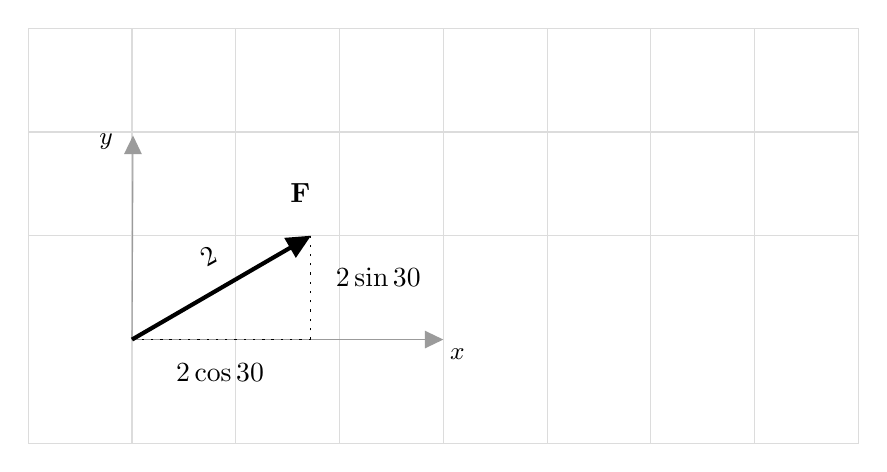
\begin{tikzpicture}[x=0.75pt,y=0.75pt,yscale=-1,xscale=1]
%uncomment if require: \path (0,201); %set diagram left start at 0, and has height of 201

%Shape: Grid [id:dp027399285057411626] 
\draw  [draw opacity=0] (0,0) -- (400,0) -- (400,200) -- (0,200) -- cycle ; \draw  [color={rgb, 255:red, 220; green, 220; blue, 220 }  ,draw opacity=1 ] (50,0) -- (50,200)(100,0) -- (100,200)(150,0) -- (150,200)(200,0) -- (200,200)(250,0) -- (250,200)(300,0) -- (300,200)(350,0) -- (350,200) ; \draw  [color={rgb, 255:red, 220; green, 220; blue, 220 }  ,draw opacity=1 ] (0,50) -- (400,50)(0,100) -- (400,100) ; \draw  [color={rgb, 255:red, 220; green, 220; blue, 220 }  ,draw opacity=1 ] (0,0) -- (400,0) -- (400,200) -- (0,200) -- cycle ;
%Straight Lines [id:da8729353257189658] 
\draw [color={rgb, 255:red, 155; green, 155; blue, 155 }  ,draw opacity=1 ][fill={rgb, 255:red, 155; green, 155; blue, 155 }  ,fill opacity=1 ]   (50,150) -- (197,150) ;
\draw [shift={(200,150)}, rotate = 180] [fill={rgb, 255:red, 155; green, 155; blue, 155 }  ,fill opacity=1 ][line width=0.08]  [draw opacity=0] (8.93,-4.29) -- (0,0) -- (8.93,4.29) -- cycle    ;
%Straight Lines [id:da5235012386016487] 
\draw [color={rgb, 255:red, 155; green, 155; blue, 155 }  ,draw opacity=1 ][fill={rgb, 255:red, 155; green, 155; blue, 155 }  ,fill opacity=1 ]   (50,150) -- (50.48,54.71) ;
\draw [shift={(50.5,51.71)}, rotate = 90.29] [fill={rgb, 255:red, 155; green, 155; blue, 155 }  ,fill opacity=1 ][line width=0.08]  [draw opacity=0] (8.93,-4.29) -- (0,0) -- (8.93,4.29) -- cycle    ;
%Straight Lines [id:da7566948648499223] 
\draw [line width=1.5]    (50,150) -- (132.71,102.01) ;
\draw [shift={(136.17,100)}, rotate = 149.87] [fill={rgb, 255:red, 0; green, 0; blue, 0 }  ][line width=0.08]  [draw opacity=0] (11.61,-5.58) -- (0,0) -- (11.61,5.58) -- cycle    ;
%Straight Lines [id:da44712188363402494] 
\draw  [dash pattern={on 0.84pt off 2.51pt}]  (136.17,150) -- (136.17,100) ;
%Straight Lines [id:da726026301324628] 
\draw  [dash pattern={on 0.84pt off 2.51pt}]  (136.17,150) -- (50,150) ;

% Text Node
\draw (202,153.4) node [anchor=north west][inner sep=0.75pt]  [font=\small]  {$x$};
% Text Node
\draw (33,49.4) node [anchor=north west][inner sep=0.75pt]  [font=\small]  {$y$};
% Text Node
\draw (125,73.4) node [anchor=north west][inner sep=0.75pt]    {$\mathbf{F}$};
% Text Node
\draw (147,114.4) node [anchor=north west][inner sep=0.75pt]    {$2\sin 30^{\degree }$};
% Text Node
\draw (70,160.4) node [anchor=north west][inner sep=0.75pt]    {$2\cos 30^{\degree }$};
% Text Node
\draw (80.07,107.24) node [anchor=north west][inner sep=0.75pt]  [rotate=-331.11]  {$2$};


\end{tikzpicture}


      \item $\bfvec{F} = 2\cos(30^\circ)\ihat + 2\sin(30^\circ)\jhat=\sqrt{3}\ihat + \jhat$, where $\cos(30^\circ)=\sqrt{3}/2$ and $\sin(30^\circ)=1/2$ was used in the last step.

    \end{enumerate}
\else



\tikzset{every picture/.style={line width=0.75pt}} %set default line width to 0.75pt        

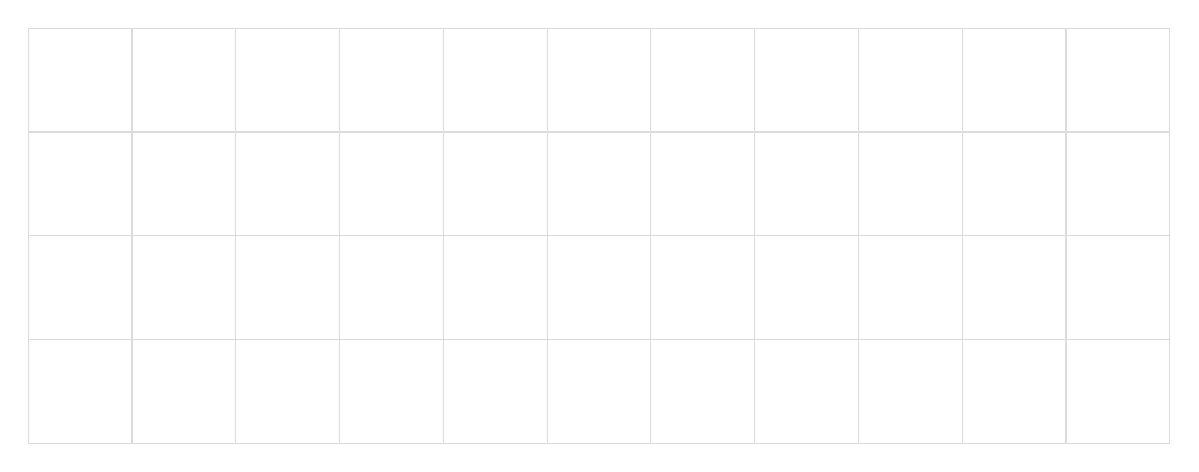
\begin{tikzpicture}[x=0.75pt,y=0.75pt,yscale=-1,xscale=1]
%uncomment if require: \path (0,208); %set diagram left start at 0, and has height of 208

%Shape: Grid [id:dp33505564538856114] 
\draw  [draw opacity=0] (2,2) -- (552,2) -- (552,202) -- (2,202) -- cycle ; \draw  [color={rgb, 255:red, 220; green, 220; blue, 220 }  ,draw opacity=1 ] (52,2) -- (52,202)(102,2) -- (102,202)(152,2) -- (152,202)(202,2) -- (202,202)(252,2) -- (252,202)(302,2) -- (302,202)(352,2) -- (352,202)(402,2) -- (402,202)(452,2) -- (452,202)(502,2) -- (502,202) ; \draw  [color={rgb, 255:red, 220; green, 220; blue, 220 }  ,draw opacity=1 ] (2,52) -- (552,52)(2,102) -- (552,102)(2,152) -- (552,152) ; \draw  [color={rgb, 255:red, 220; green, 220; blue, 220 }  ,draw opacity=1 ] (2,2) -- (552,2) -- (552,202) -- (2,202) -- cycle ;




\end{tikzpicture}

\fi

\section{Problem II}

Given $\bfvec{F}=3\ihat - 4\jhat$,

\begin{enumerate}

  \item Draw $\bfvec{F}$.

  \item Compute $F$.

  \item The angle  $\bfvec{F}$ makes with respect to the $x$--axis (with positive rotation counterclockwise).

\end{enumerate}

\ifsolutions
\textbf{Solution}

    \begin{enumerate}

      \item 

            

\tikzset{every picture/.style={line width=0.75pt}} %set default line width to 0.75pt        

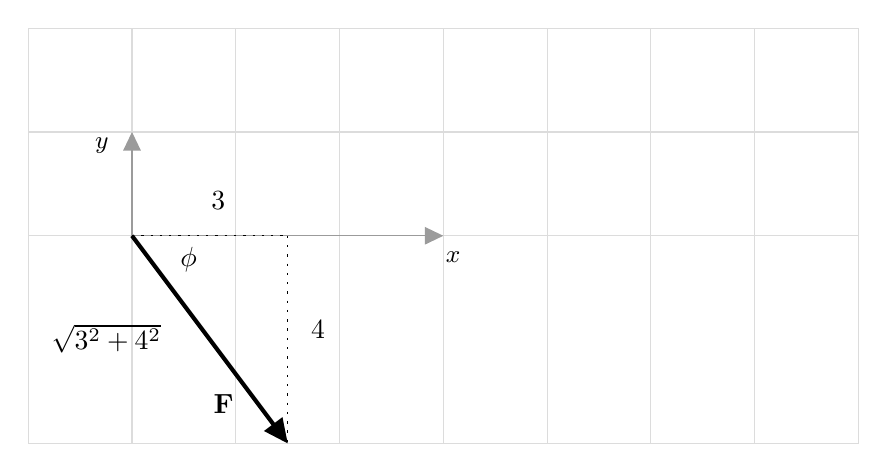
\begin{tikzpicture}[x=0.75pt,y=0.75pt,yscale=-1,xscale=1]
%uncomment if require: \path (0,201); %set diagram left start at 0, and has height of 201

%Shape: Grid [id:dp7678677023018607] 
\draw  [draw opacity=0] (0,-50) -- (400,-50) -- (400,150) -- (0,150) -- cycle ; \draw  [color={rgb, 255:red, 220; green, 220; blue, 220 }  ,draw opacity=1 ] (50,-50) -- (50,150)(100,-50) -- (100,150)(150,-50) -- (150,150)(200,-50) -- (200,150)(250,-50) -- (250,150)(300,-50) -- (300,150)(350,-50) -- (350,150) ; \draw  [color={rgb, 255:red, 220; green, 220; blue, 220 }  ,draw opacity=1 ] (0,0) -- (400,0)(0,50) -- (400,50) ; \draw  [color={rgb, 255:red, 220; green, 220; blue, 220 }  ,draw opacity=1 ] (0,-50) -- (400,-50) -- (400,150) -- (0,150) -- cycle ;
%Straight Lines [id:da04962468288547894] 
\draw [color={rgb, 255:red, 155; green, 155; blue, 155 }  ,draw opacity=1 ][fill={rgb, 255:red, 155; green, 155; blue, 155 }  ,fill opacity=1 ]   (50,50) -- (197,50) ;
\draw [shift={(200,50)}, rotate = 180] [fill={rgb, 255:red, 155; green, 155; blue, 155 }  ,fill opacity=1 ][line width=0.08]  [draw opacity=0] (8.93,-4.29) -- (0,0) -- (8.93,4.29) -- cycle    ;
%Straight Lines [id:da3237467676353869] 
\draw [color={rgb, 255:red, 155; green, 155; blue, 155 }  ,draw opacity=1 ][fill={rgb, 255:red, 155; green, 155; blue, 155 }  ,fill opacity=1 ]   (50,50) -- (50,3) ;
\draw [shift={(50,0)}, rotate = 90] [fill={rgb, 255:red, 155; green, 155; blue, 155 }  ,fill opacity=1 ][line width=0.08]  [draw opacity=0] (8.93,-4.29) -- (0,0) -- (8.93,4.29) -- cycle    ;
%Straight Lines [id:da7090426014185081] 
\draw  [dash pattern={on 0.84pt off 2.51pt}]  (125,50) -- (125,150) ;
%Straight Lines [id:da029077223942405306] 
\draw [line width=1.5]    (50,50) -- (122.6,146.8) ;
\draw [shift={(125,150)}, rotate = 233.13] [fill={rgb, 255:red, 0; green, 0; blue, 0 }  ][line width=0.08]  [draw opacity=0] (11.61,-5.58) -- (0,0) -- (11.61,5.58) -- cycle    ;
%Straight Lines [id:da08836194799357244] 
\draw  [dash pattern={on 0.84pt off 2.51pt}]  (50,50) -- (125,50) ;

% Text Node
\draw (200,56.4) node [anchor=north west][inner sep=0.75pt]  [font=\small]  {$x$};
% Text Node
\draw (31,1.4) node [anchor=north west][inner sep=0.75pt]  [font=\small]  {$y$};
% Text Node
\draw (88,125.4) node [anchor=north west][inner sep=0.75pt]    {$\mathbf{F}$};
% Text Node
\draw (135,89.4) node [anchor=north west][inner sep=0.75pt]    {$4$};
% Text Node
\draw (87,27.4) node [anchor=north west][inner sep=0.75pt]    {$3$};
% Text Node
\draw (10,91.4) node [anchor=north west][inner sep=0.75pt]    {$\sqrt{3^{2} +4^{2}}$};
% Text Node
\draw (72,54.4) node [anchor=north west][inner sep=0.75pt]    {$\phi $};


\end{tikzpicture}


      \item $F=\sqrt{3^2+4^2}=5$

      \item $\ds\theta = 360^\circ - \phi = 360^\circ - \frac{180}{\pi}\tan^{-1}(4/3)\simeq 307^\circ$

    \end{enumerate}
\else



\tikzset{every picture/.style={line width=0.75pt}} %set default line width to 0.75pt        

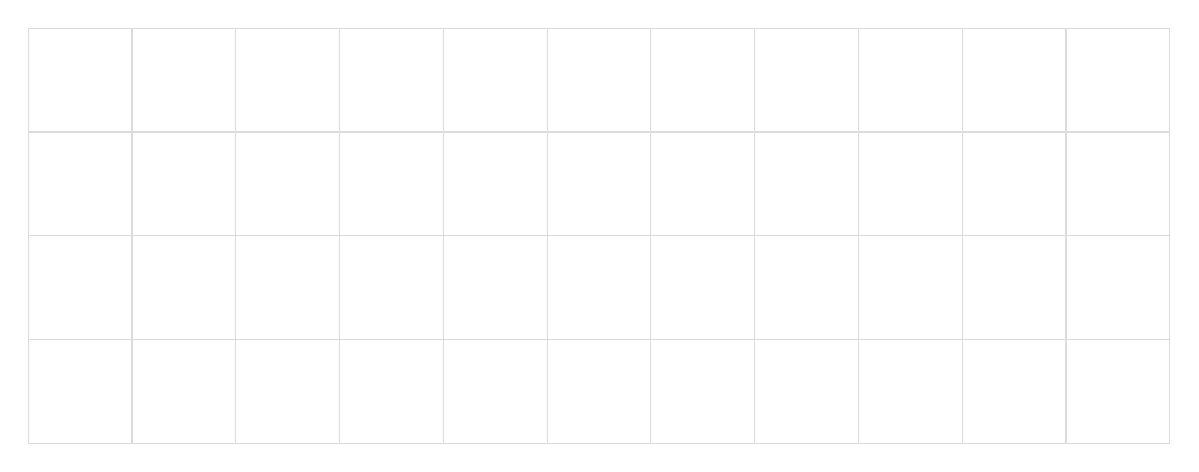
\begin{tikzpicture}[x=0.75pt,y=0.75pt,yscale=-1,xscale=1]
%uncomment if require: \path (0,208); %set diagram left start at 0, and has height of 208

%Shape: Grid [id:dp33505564538856114] 
\draw  [draw opacity=0] (2,2) -- (552,2) -- (552,202) -- (2,202) -- cycle ; \draw  [color={rgb, 255:red, 220; green, 220; blue, 220 }  ,draw opacity=1 ] (52,2) -- (52,202)(102,2) -- (102,202)(152,2) -- (152,202)(202,2) -- (202,202)(252,2) -- (252,202)(302,2) -- (302,202)(352,2) -- (352,202)(402,2) -- (402,202)(452,2) -- (452,202)(502,2) -- (502,202) ; \draw  [color={rgb, 255:red, 220; green, 220; blue, 220 }  ,draw opacity=1 ] (2,52) -- (552,52)(2,102) -- (552,102)(2,152) -- (552,152) ; \draw  [color={rgb, 255:red, 220; green, 220; blue, 220 }  ,draw opacity=1 ] (2,2) -- (552,2) -- (552,202) -- (2,202) -- cycle ;




\end{tikzpicture}

\fi

\end{document}